\documentclass[14pt, aspectratio=169]{beamer}
\usepackage{unicode}
\usepackage{apacite}
\usepackage{parskip}
\usepackage{listings}
\usepackage{times}
\usepackage{tabularx}
\usepackage{tikz}
\usepackage{mdframed}
\usepackage{caption}
\usepackage{rotating}
\newcommand {\scaledimage}[1] {
    \includegraphics[width=\textwidth,height=0.8\textheight,keepaspectratio]{#1}
}
\usetikzlibrary{positioning,arrows,automata}

\setbeamertemplate{navigation symbols}{}
\title{Especificación del Analizador Léxico}
\author{Aramis E. Matos, Lenier Gerena, Angel Berrios Pellot}

\usetheme{Berlin}
\usecolortheme{beaver}


\begin{document}
\maketitle
\begin{frame}{Introduccion}
    \small Escribir Introduccion 
\end{frame}

\begin{frame}{Objetivo}
    \small Escrirbir objetivos 
\end{frame}

\begin{frame}{Indice}
    \item Tabla simbolos
    \item Diseño de analizador lexico
    \item Especificaciones  
    \begin{itemize}
        \item token
        \item patron
        \item lexema
        \item atributos
    \end{itemize}
\end{frame}

\begin{frame}{Indice}
    \item Expreciones regulares / AFN
    \item tabla de transiciones 
    \item seguir añadiendo
\end{frame}

\begin{frame}[fragile=singleslide]
    \frametitle{Code}
    \small
closeToZero = take 100 \$ map(\\x -> 1 / powerDouble 10 x)[1.0 ..]

closeToDoubleLimit = [maxBound - 99 .. maxBound] :: [Int]

turnToDouble x = read (filter (/= 'n') x) :: Double

\end{frame}

\begin{frame}{Tabla de Simbolos}
    
\begin{table}[ht]
    \footnotesize
    \begin{tabularx}{\linewidth}{|X|X|X|X|}
        \hline
        Lexema & \textit{Token}        & Patrones                                                              & Atributo                                          \\\hline
        ;      & <FIN\_DE\_ LINEA>     & ; | :                                                                 & Indica fin de Línea                               \\\hline
        defina & <PALABRA\_ RESERVADA> & defina | como                                                         & Indica declaración de una variable                \\\hline
        VaR1   & <ID>                  & [A-Za-z] | <LETRA> <IDCONT>                                           & Apuntador a la tabla de símbolos                  \\\hline
        X1     & <IDCONT>              & \textit{[A-Za-z]} | <LETRA> <IDCONT> | \textit{[0-9]} | <DIGITO> <IDCONT> & Permite que los identificadores contengan números \\\hline
    \end{tabularx}
    \label{table: lexTable1}
    \caption{Definición Léxica del Lenguaje AVISMO}
\end{table}
\end{frame}

\begin{frame}{Tabla de Simbolos}

\begin{table}[ht]
    \footnotesize
    \begin{tabularx}{\linewidth}{|X|X|X|X|}
        \hline
        =      & <ASIGNACION>          & =                                                                     & Asigna un <MODELO\_MOLECULAR a un identificador   \\\hline
        X1y2   & <ID>                  & [A-Za-z] | <LETRA> <IDCONT>                                           & Indica declaración de una variable                \\\hline
        A      & <LETRA>               & [A-Za-z]                                                              & Provee un terminal para <ID> y <IDCONT>           \\\hline
        1      & <DIGITO>              & [0-9]                                                                 & Escribir algo                                     \\\hline
    \end{tabularx}
    \label{table: lexTable2}
    \caption{Definición Léxica del Lenguaje AVISMO}
\end{table}
\end{frame}

\begin{frame}{Diseño del Analizador Léxico}
    \begin{figure}[ht]
    \footnotesize
        \begin{minipage}{.4\textwidth}
            \centering
            \begin{mdframed}
                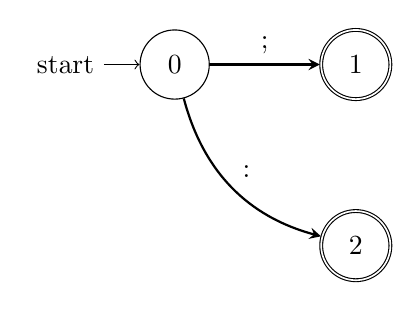
\begin{tikzpicture}[node distance = 2.3cm, on grid, auto]
                    \node [state,initial] (q0) {$0$};
                    \node [state,accepting] [right=of q0] (q1) {$1$};
                    \node [state,accepting] [below=of q1] (q2) {$2$};
    
                    \path[-stealth, thick]
                    (q0) edge node {;} (q1)
                    (q0) edge [bend right] node {:} (q2);
                \end{tikzpicture}
                \label{fig: finDeLineaAutomata}
            \end{mdframed}
            \caption{Automata del patrón para el token <FIN\_DE\_LINEA>}
        \end{minipage}\hspace{1cm}
        \begin{minipage}{0.4\textwidth}
            \centering
            \begin{mdframed}
                \begin{tikzpicture}[node distance = 2.3cm, on grid, auto]
                    \node [state, initial] (q0) {$0$};
                    \node [state, accepting] [right=of q0] (q1) {$1$};
                    \node [state, accepting] [below=of q1] {$1$};
    
                    \path[-stealth, thick]
                    (q0) edge node {defina} (q1)
                    (q0) edge [bend right] node {como} (q2);
                \end{tikzpicture}
            \end{mdframed}
            \label{fig: palabraReservada}
            \captionof{figure}{Automata del patrón para el token <PALABRAS\_RESERVADA>}
        \end{minipage}
    \end{figure}
\end{frame}

\begin{frame}
    \begin{figure}[ht]
        \footnotesize
        \begin{minipage}{0.41\textwidth}
            \begin{mdframed}
                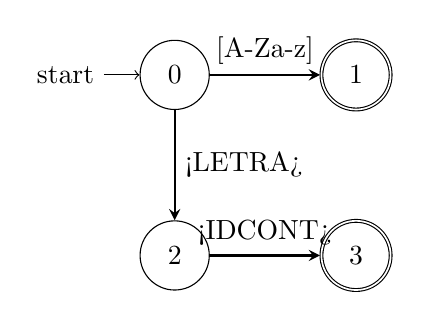
\begin{tikzpicture}[node distance = 1.4cm, auto]
                    \node [state, initial] (q0) {0};
                    \node [state, accepting] [right=of q0] (q1) {$1$};
                    \node [state] [below=of q0] (q2) {$2$};
                    \node [state, accepting] [right=of q2] (q3) {$3$};
    
                    \path[-stealth, thick]
                    (q0) edge node {[A-Za-z]} (q1)
                    (q0) edge node {<LETRA>} (q2)
                    (q2) edge node {<IDCONT>} (q3);
                \end{tikzpicture}
            \end{mdframed}
            \label{fig: idAutomata}
            \caption{Automata del patrón para el token <ID>}
        \end{minipage}\hspace{1cm}
    \end{figure}
\end{frame}

\begin{frame}
    \begin{figure}[ht]
        \footnotesize
        \begin{minipage}{0.5\textwidth}
            \begin{mdframed}
                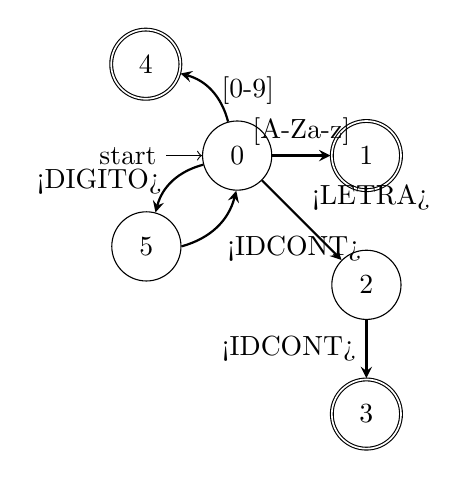
\begin{tikzpicture}[node distance = 21pt, auto]
                    \node [state, initial] (q0) {$0$};
                    \node [state, accepting] [right=of q0] (q1) {$1$};
                    \node [state] [below=of q1] (q2) {$2$};
                    \node [state, accepting] [below=of q2] (q3) {$3$};
                    \node [state, accepting] [above left=of q0] (q4) {$4$};
                    \node [state] [below left=of q0] (q5) {$5$};
                    
    
                    \path[-stealth, thick]
                    (q0) edge node {[A-Za-z]} (q1)
                    (q0) edge node {<LETRA>} (q2)
                    (q2) edge node [left] {<IDCONT>} (q3)
                    (q0) edge [bend right] node[right] {[0-9]} (q4)
                    (q0) edge [bend right] node [left] {<DIGITO>} (q5)
                    (q5.east) edge [bend right] node [below right] {<IDCONT>} (q0);
    
                    
                \end{tikzpicture}
            \end{mdframed}
            \label{fig: idContAutomata}
            \caption{Automata del patrón para el token <IDCONT>}
        \end{minipage}
    \end{figure}
\end{frame}

\begin{frame}
    \begin{figure}[ht]
        \footnotesize
        \begin{minipage}{0.5\textwidth}
            \begin{mdframed}
                \begin{tikzpicture}[node distance = 0cm, auto]
                    \node [state,initial] (q0) {$0$};
                    \node [state,accepting] [right=of q1] (q1) {$1$};
    
                    \path[-stealth,thick]
                    (q0) edge node {=} (q1);
                \end{tikzpicture}
            \end{mdframed}
            \label{fig: asigAutomata}
            \caption{Automata del patrón para el token <ASIGNACION>}
        \end{minipage}\hspace{1cm}
        \begin{minipage}{0.5\linewidth}
            \begin{mdframed}
                \begin{tikzpicture}[node distance = 0cm, on grid ,auto]
                    \node [state,initial] (q0) {$0$};
                    \node [state,accepting] [right=of q1] (q1) {$1$};
    
                    \path[-stealth,thick]
                    (q0) edge node {[0-9]} (q1);
                \end{tikzpicture}
            \end{mdframed}
            \label{fig: letraAutomata}
            \caption{Automata del patrón para el token <LETRA>}
        \end{minipage}
    \end{figure}
\end{frame}

\begin{frame}{Big Chungus}
    \cite{narciso_farias_gramatica_2012}

    \cite{tapkeer_flex_2023}
\end{frame}

\begin{frame}[allowframebreaks]
    \frametitle{Referencias}
    \bibliography{../../report/References}
    \bibliographystyle{apacite}
\end{frame}


\end{document}